% !TeX spellcheck = en_US
\addsection{Other Rules}{\skills/armorer.png}
\begin{multicols}{2}

\subsection*{\hypertarget{Trading}{Trading}}\index{Trading}

The \hyperlink{Trading Post}{Trading Post Field} and other effects allow you to trade Resources with the game in accordance to the table below.
You may also \textbf{Remove cards} from your hand at the trading post to gain 1 \includesvg[height=10px]{\svgs/gold.svg} per card.\par
\note{5}{Specialty, Statistic, Starting Ability and Magic Arrows \textbf{cannot be removed} in the Trading Post.}\par
In \textbf{Alliance} and \textbf{Cooperative} Scenarios, players are allowed to trade Resources and cards following these rules:
\begin{itemize}
  \item In Alliance Scenarios, allies may trade Resources freely at any time on their Turns except during Combat.
  \item In Cooperative Scenarios, Resources may be given to other players when Visiting a Trading Post.
  \item In both Scenario types, allies may trade \textbf{Spell} and \textbf{Artifact} cards in any mix if they have heroes on adjacent Fields.
    Only \textbf{cards from their hands} may be traded and you must give and receive an equal amount of cards.
\end{itemize}

\vspace*{\fill}
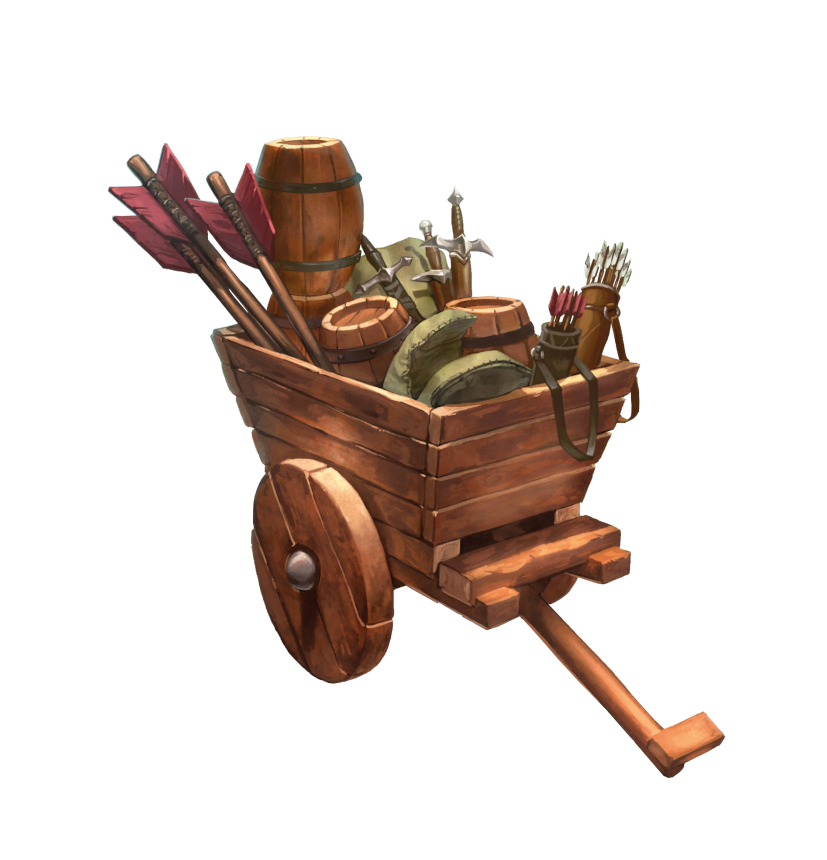
\includegraphics[width=\linewidth]{\art/ammo_cart.png}

\end{multicols}

\vfill
\begin{figure*}[!hb]
  \centering
  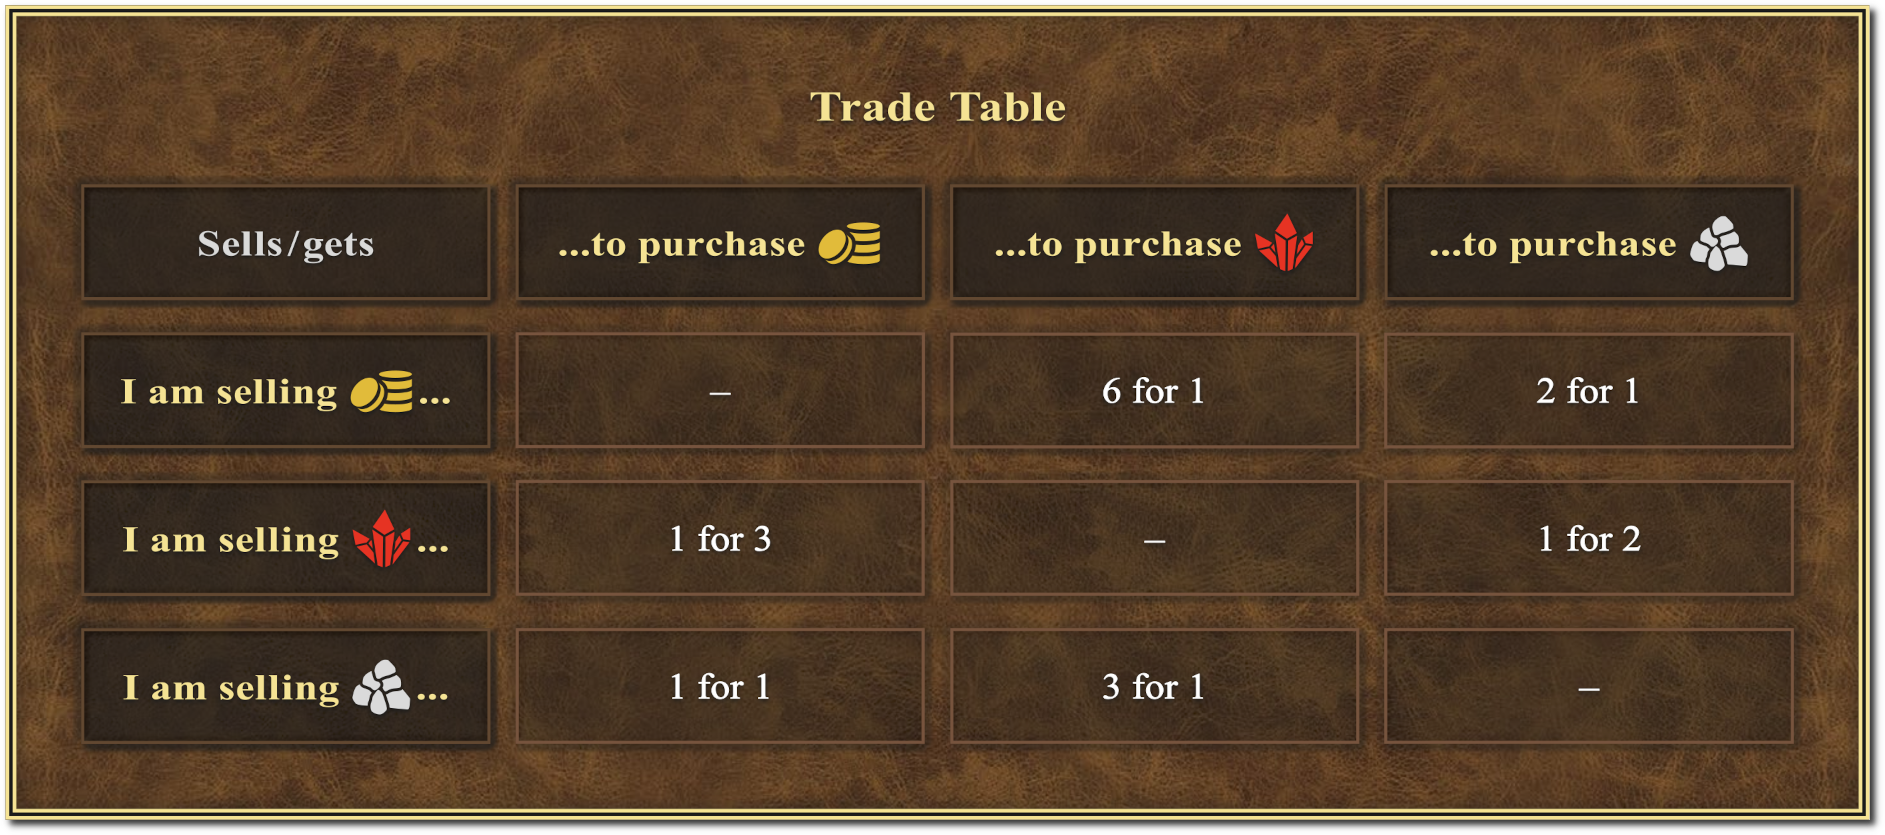
\includegraphics[width=\linewidth]{\tables/trade_table.png}
\end{figure*}
\vfill
